\section{Results}

\subsection{Coincidence-to-accidentals ratio}
One issue that must be addressed when determining the statistics of the different parameters is that the \acrfull{car} depends on the exposure time. Therefore, before measuring the statistical distributions, an exposure time must be found for which the \acrshort{car} value remains constant. Thus, this value was measured for nine exposure times ranging from ten milliseconds to sixty seconds. The integration time was set to ten times the exposure time for each measurement. Hence, ten histograms were saved for each exposure time and based on these histograms, the average \acrshort{car} value and its standard deviation were calculated. \newline
The results are shown in \autoref{fig:CAR}. As the exposure time increases, it can be seen that the fluctuation of the \acrshort{car} value, i.e. its standard deviation, decreases. Furthermore, after an exposure time of one second, the \acrshort{car} value remains approximately constant. Therefore, this range from one second onwards is preferred for statistical analysis. However, as this requires many consecutive and lengthy measurements, the aim is to use the shortest possible exposure time at which the \acrshort{car} value remains constant. Therefore, one second will be used as the exposure time for upcoming measurements.
\begin{figure}[bt!]
	\centering
	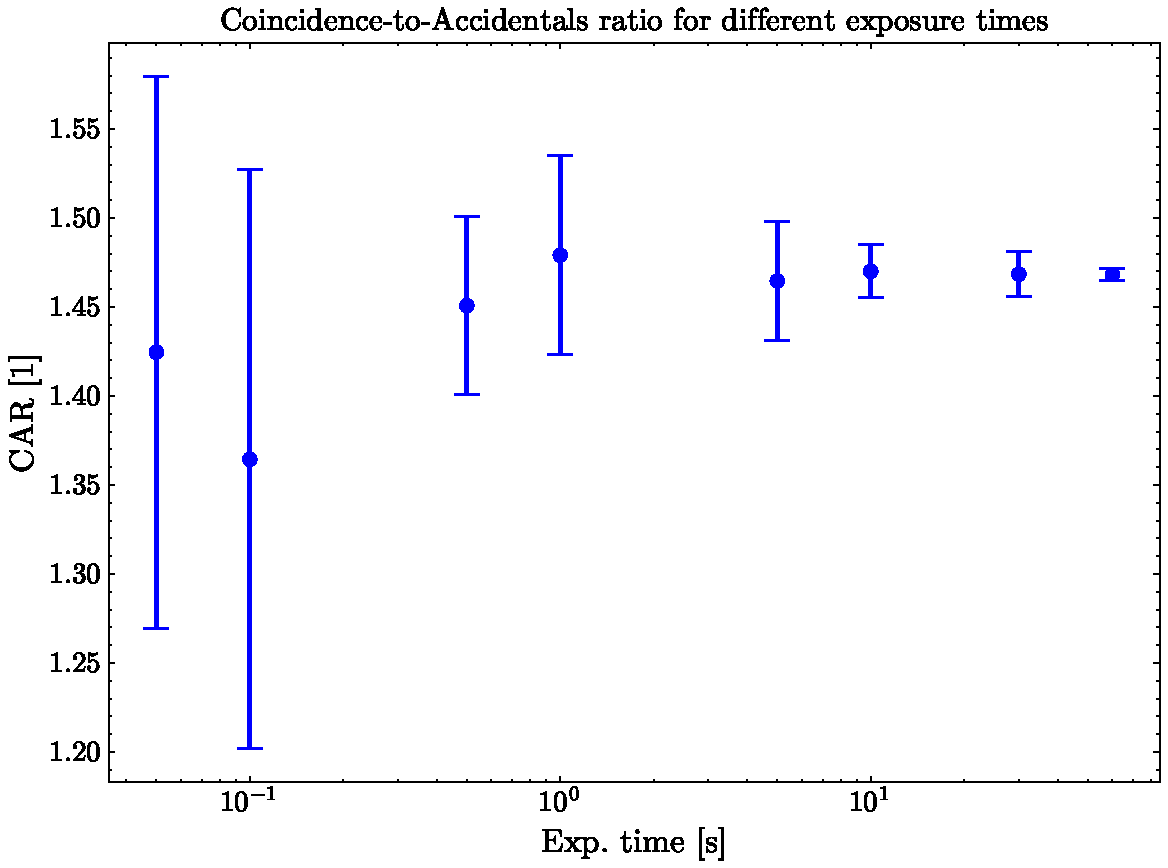
\includegraphics[width=.7\textwidth]{Images/CAR_Ratio.pdf}
	\caption{Coincidence-to-Accidentals ration for different exposure times}
	\label{fig:CAR}
\end{figure}
\subsection{Dark counts}
The first parameter to be determined is the statistical distribution of dark counts in both arms. This result is necessary for obtaining the variance of noise in the conventional approach in \autoref{eq:VarianceTransExpl}. For the measurement, the exposure time was set to one second, and the integration time was set to one thousand seconds. To obtain the intrinsic dark counts, both single-photon detectors were disconnected from the setup and the measurement was repeated five times. \newline
The measurement results for the idler arm can be seen in \autoref{fig:DCIdl}. It shows the probability distribution for each dark count rate. Additionally, a Poisson distribution was fitted to the experimental data with the same average count rate. This was done because it is expected that the dark counts of single-photon detectors will exhibit a Poisson distribution \cite{foucheDetectionFalsealarmProbabilities2003}. However, the two distributions do not match, indicating that the experimentally obtained data does not follow a Poisson distribution. This is also confirmed by calculating the variance-to-mean ratio, which, in the case of a Poisson distribution, should equal one. The ratio was calculated for each of the five repeats and averaged to 1.78. This is shown in the black box of \autoref{fig:DCIdl}. 
\begin{figure}[tb!]
	\centering
	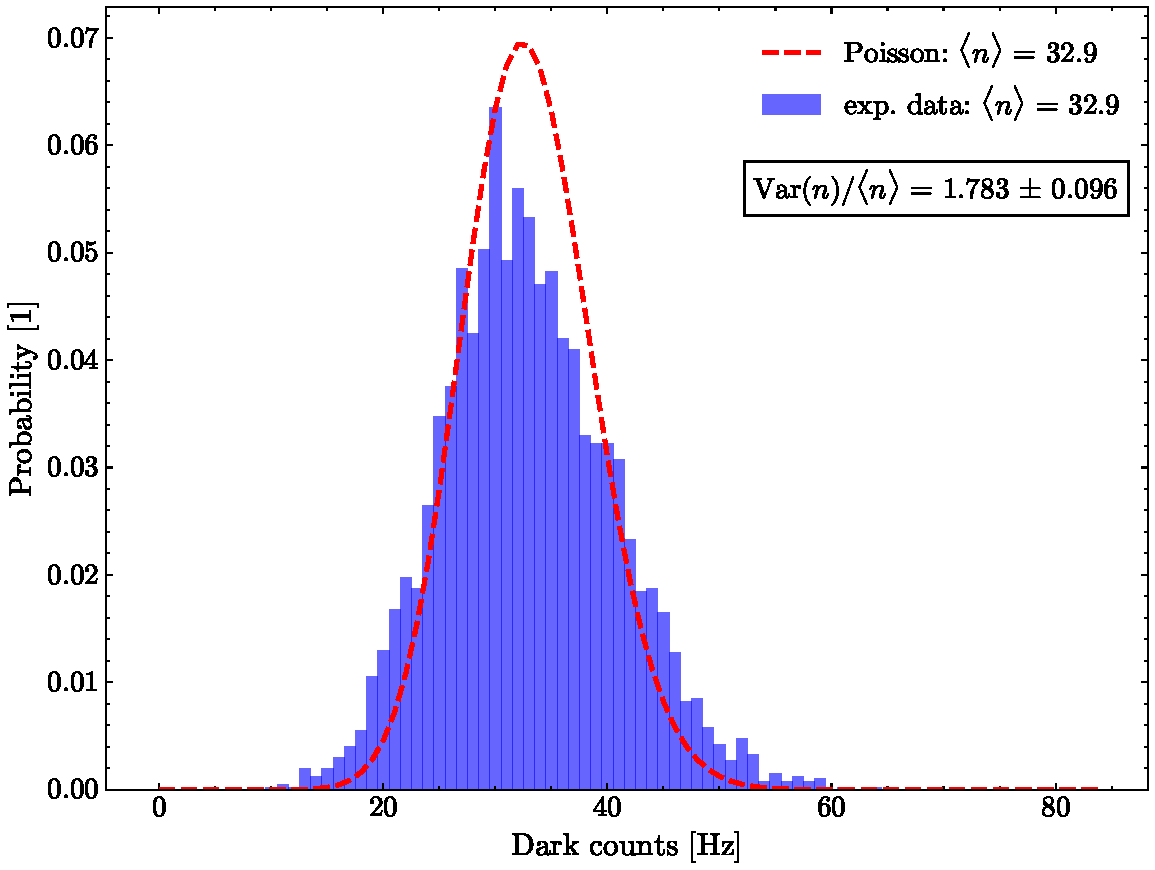
\includegraphics[width=.7\textwidth]{Images/DC_Idl.pdf}
	\caption{Dark counts of the IR single photon detector in the idler arm}
	\label{fig:DCIdl}
\end{figure}\newline
This mismatch may be caused by the afterpulsing effect. This effect refers to spurious detection events that occur shortly after genuine photon detection, even though no new photons have arrived. These false counts arise from trapped charge carriers released after the detector resets, triggering a secondary avalanche. This effect is well-known in InGaAs single-photon detectors operating in the infrared, such as the one used in this experiment \cite{laiImpactAfterpulsingEffects2024}. Consequently, this effect introduces correlations between detection events that, according to Poisson statistics, should be independent and artificially increases the count rate. Therefore, the variance of counts is larger than expected for a Poisson process. \newline
A strong indication that the mismatch is caused by afterpulsing is that the probability of afterpulsing events decreases exponentially with the detector's dead time. Since individual afterpulses could not be measured directly, the variance-to-mean ratio was measured instead. As the number of correlated events decreases as the probability of afterpulsing decreases, the variance-to-mean ratio should also decrease and approach one, as in a Poisson distribution \cite{humerSimpleRobustMethod2015}. The exponential decay of the variance-to-mean ratio is shown in the appendix in \autoref{fig:VoMDead}, thus confirming that the mismatch is caused by afterpulsing. \newline
For the analysis of the dark counts in the signal arm, which are in the visible range, the same experimental settings as for the idler arm were used. The statistical distribution of the dark counts in the signal arm can be seen in \autoref{fig:DCSig}.
\begin{figure}[tb!]
	\centering
	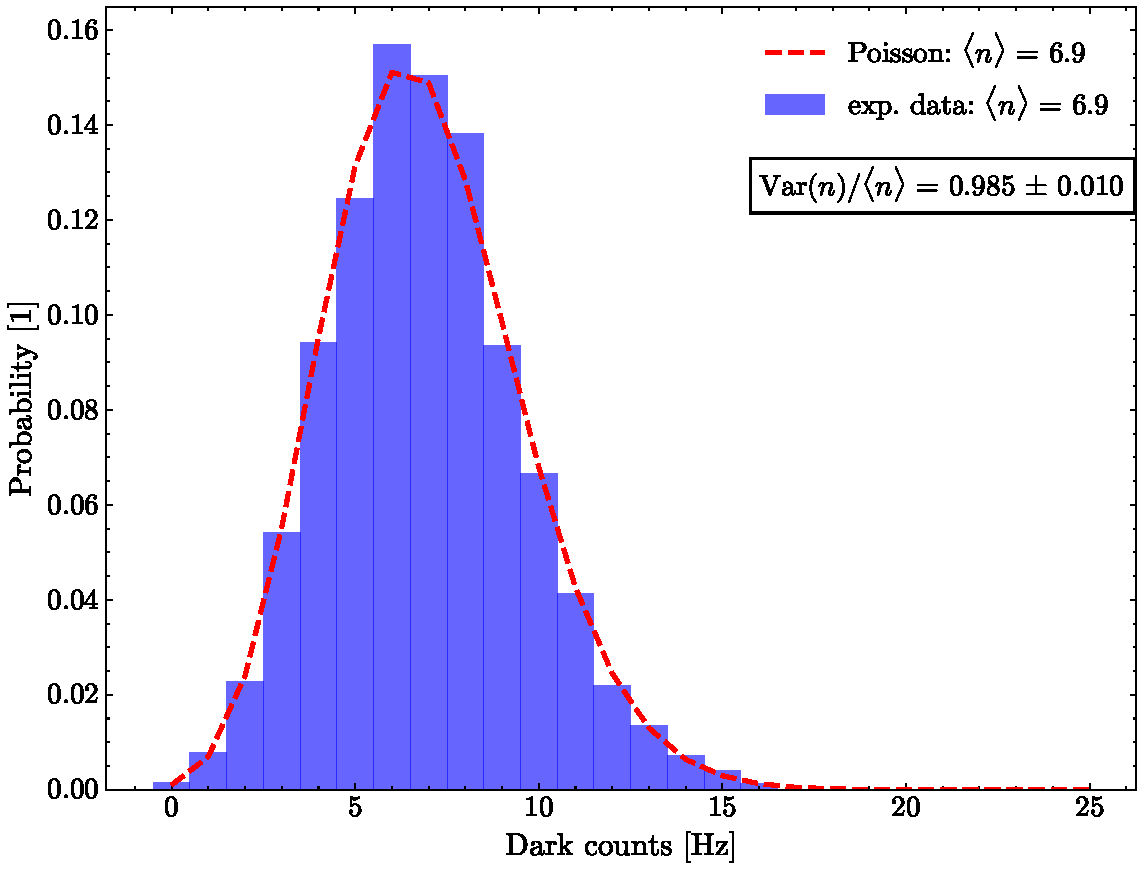
\includegraphics[width=.7\textwidth]{Images/DC_Sig.pdf}
	\caption{Dark counts of the VIS single photon detector in the signal arm}
	\label{fig:DCSig}
\end{figure}
As for the idler arm, a Poissonian fit was added to the figure. This shows that the distribution of dark counts matches the Poisson distribution very well. It is confirmed by considering the variance-to-mean ratio of the counts, shown in the black box, which was calculated for each of the five repeats. On average, it yields 0.985, indicating that it can be well approximated by a Poisson distribution.


\begin{comment}
	
	
	\begin{figure}
		\noindent
		\begin{minipage}{0.33\textwidth}
			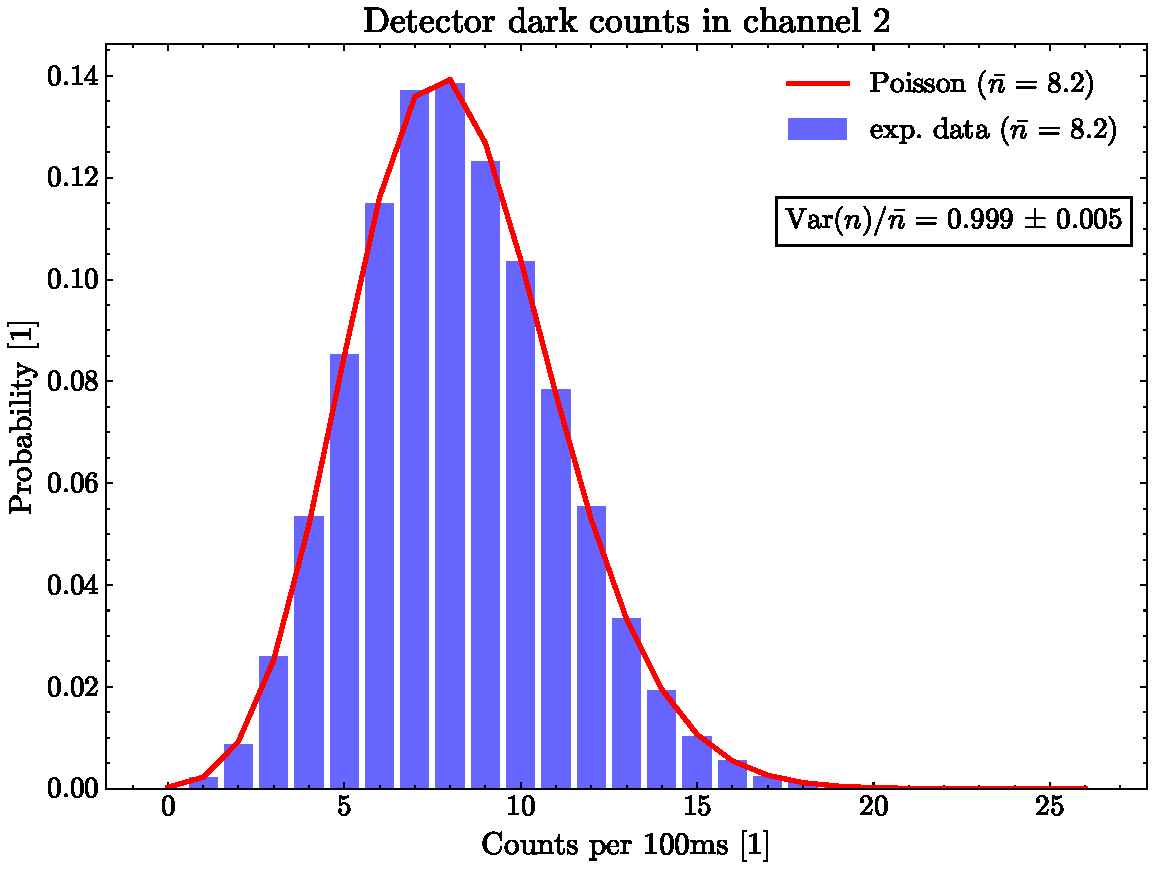
\includegraphics[page=1,width=\linewidth]{Images/DC_chAll.pdf}
		\end{minipage}%
		\begin{minipage}{0.33\textwidth}
			\includegraphics[page=2,width=\linewidth]{Images/DC_chAll.pdf}
		\end{minipage}%
		\begin{minipage}{0.33\textwidth}
			\includegraphics[page=3,width=\linewidth]{Images/DC_chAll.pdf}
		\end{minipage}
		\caption{TestCap}
		\label{fig:DC}
	\end{figure}
\end{comment}
\subsection{Single counts}


To correctly model \autoref{eq:VarianceTransExpl} and the variance of the total photon counts (i.e.,$\operatorname{Var}\!\left( N_{\text{tot}}^{\text{ref}} \right)$ and $\operatorname{Var}\!\left( N_{\text{tot}}^{\text{sam}} \right)$), the statistics of the idler arm were investigated experimentally. \newline
For the measurement, the exposure time was set to one second and the integration time to one thousand seconds. Thus, each measurement yielded 1,000 data points for statistical analysis. The measurement was repeated five times to account for statistical fluctuations and determine an interval for the variance-to-mean ratio.
The results of the measurements are shown in \autoref{fig:StatIdl}. \newline
The average photon number $\langle n\rangle$ is 65,107. Furthermore, the mode number $m_{theo}$, which was determined using the experimental variance value and \autoref{eq:VariancemmBE}, is 61,384. Based on these two values, a \acrshort{mmbe} and a Poisson distribution were modeled. As can be seen, the Poisson distribution significantly overestimates the peak of the experimental distribution. Additionally, the Poisson distribution decreases faster than the experimental distribution, so the edges of the distribution are not modeled correctly. On the other hand, the \acrshort{mmbe} fit agrees much better with the experimental distribution because it properly estimates the peak and the edges of the experimental distribution fall within the theoretical fit.
\begin{figure}[tb!]
	\centering
	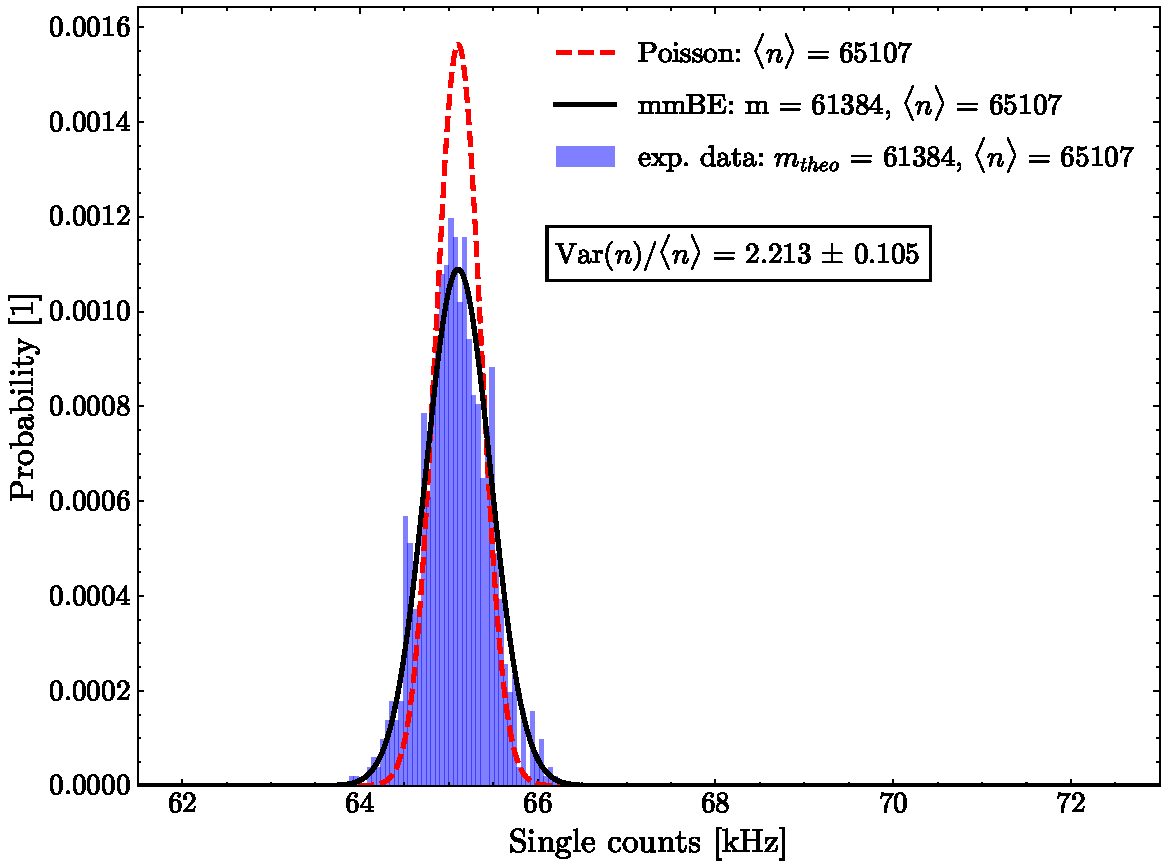
\includegraphics[width=.7\textwidth]{Images/SingleStatisticsIdler.pdf}
	\caption{Photon statistics in the idler arm}
	\label{fig:StatIdl}
\end{figure}\newline
The black box shows the variance-to-mean ratio for the five repeated measurements. The mean value is 2.2, with a standard deviation of 0.1. Since this ratio is not equal to one, it confirms that the experimental distribution is not Poisson but has a higher variance. For the modeling of the variance of the single counts, this means that $\operatorname{Var}\!\left( N_{\text{tot}}^{\text{ref}} \right)$ and $\operatorname{Var}\!\left( N_{\text{tot}}^{\text{sam}} \right)$ can be approximated by the mean photon number multiplied with a factor of 2.2. \newline
As a consistency check, the statistics of the photons in the signal arm were also measured, as they should exhibit a \acrshort{mmbe} distribution. The experimental parameters are kept the same as in the idler arm measurements. \newline
The results can be seen in \autoref{fig:StatSig}. The approach for calculating the Poisson and \acrshort{mmbe} distribution is the same as for the idler photons. Similar to the idler arm, the \acrshort{mmbe} model more closely resembles the experimental distribution than the Poisson model because it overestimates the peak and underestimates the edges of the distribution. This is confirmed once more by calculating the variance-to-mean ratio, which yields an average of 1.9 and shows that the distribution is not Poissonian. \newline
The count rate of the signal photons is roughly 30 times higher than the idler photons. One reason for this may be that the idler photon spectrum is much broader than the signal's. Consequently, the spatial cone of the emitted idler photons is larger. The focusing lens may have a smaller clear aperture than the spatial extent of the cone, resulting in some photons being clipped. Meanwhile, the focusing lens in the signal arm collects the entire spectrum. Another reason may be that, due to the broader spectrum in the idler arm, the chromatic aberration of the lens leads to different focal lengths, so not the entire spectrum is coupled into the fiber. \newline
Since the mode number ($m_{theo}$) is directly related to the average photon number, a high count rate also results in a significantly larger mode number.
\todo[inline]{Can I calculate $m_{theo}$ in another way??}
\begin{figure}[tb!]
	\centering
	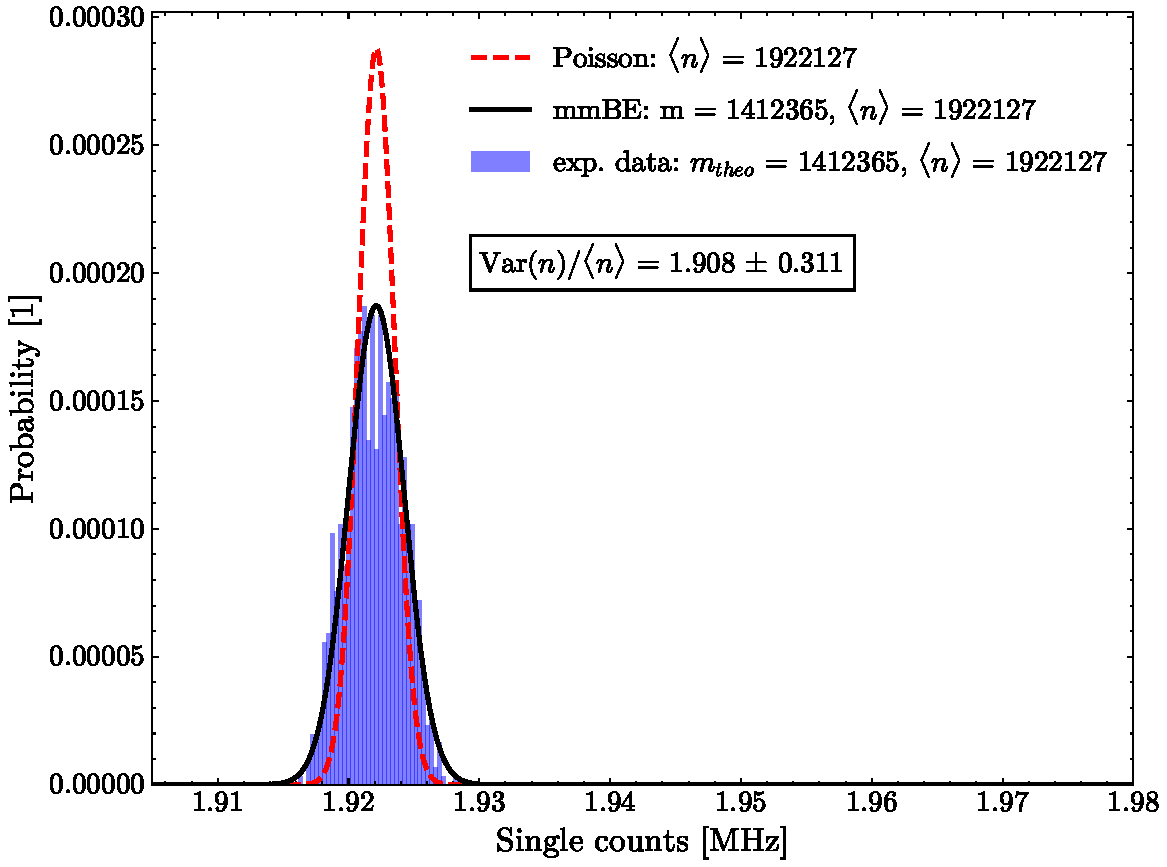
\includegraphics[width=.7\textwidth]{Images/SingleStatisticsSignal.pdf}
	\caption{Photon statistics in the signal arm}
	\label{fig:StatSig}
\end{figure}

\subsection{Coincidence counts}
To determine the statistics of the coincidence counts that are required to calculate the variance of the transmittance in \autoref{eq:VarianceTransExplCoinc}, five measurements were performed. The experimental parameters were kept the same as in the previous section for the singles. Therefore, an exposure time of one second and an integration time of one thousand seconds was used. For every step in time, a histogram was saved by the time-tagging unit. The bin width was set to 4.68 ns and the number of bins to 200. The coincidence window was set to $\tau_{\text{cw}} = $ 9.36 ns, which means that two bins were selected as coincidence counts.\newline
The results of the measurements are shown in \autoref{fig:StatCoinc}. Similarly to the single counts, a Poisson distribution is modeled based on the average photon counts observed in the experiment. As can be seen, the experimental distribution is well approximated by the Poisson distribution. This is confirmed by considering the variance-to-mean ratio illustrated in the black box. An average value of 1.040 and a standard deviation of 0.035 are achieved for the five measurements. This coincides with the theoretical prediction in \autoref{sec:cohLight} that coincidence counts can be approximated by a Poisson distribution where the variance equals the mean. \newline
Consequently, the variance of the coincidence counts in the model for the simulation can be substituted by the average coincidence counts.
\begin{figure}[tb!]
	\centering
	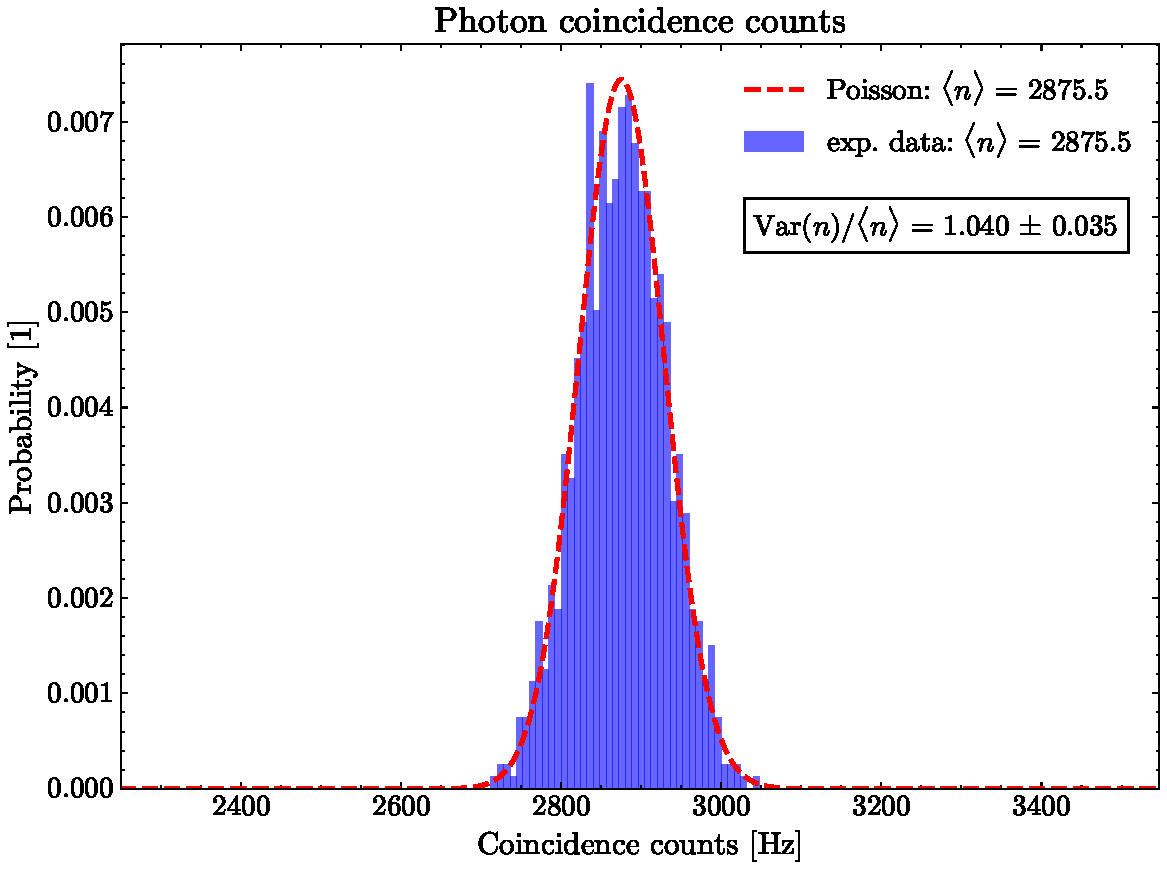
\includegraphics[width=.7\textwidth]{Images/CoincStatistics.pdf}
	\caption{Photon statistics of coincidence counts}
	\label{fig:StatCoinc}
\end{figure}

\subsection{Accidental counts}
Regarding accidental counts, two parameters have to be determined experimentally.
Not only must the variance of the accidental counts be measured for \autoref{eq:VarianceTransExplCoinc}, but also \autoref{eq:AccCounts} for calculating them from single and coincidence counts. \newline
For the variance measurement, the exposure time was set to one second and the integration time to sixty seconds.
The histogram of the coincidences was used to retrieve the accidental counts. The bin width was set to 1.4 ns and the number of bins to 110. The coincidence window was set to 2.8 ns, which means that two bins were selected as coincidence counts. A representative histogram can be seen in appendix in \autoref{fig:HistExamAcc}.
%To obtain just the accidental counts from each histogram, not only the two coincidence peaks, but also the two adjacent bins were neglected. This results in 6,300 accidental counts over the sixty time steps.
\newline
The statistical distribution is shown in \autoref{fig:StatAcc}. Similar to previous results, a Poisson distribution was modeled based on average accidental counts. As can be seen, the Poissonian fit closely matches the experimental distribution. \newline
To obtain a quantitative measure of the distribution in addition to a qualitative one, the variance-to-mean ratio was again calculated. For each time step, 105 values were obtained for the accidental counts, and the variance-to-mean ratio was determined. Then, the average and standard deviation of the ratio were calculated for the sixty steps. The result is shown in the black box of \autoref{fig:StatAcc}. \newline
Within the limits of the standard deviation, the ratio corresponds to one, which is the ratio of a Poisson distribution. Therefore, the accidental counts can be assumed to have a Poisson distribution, and the variance can be substituted by the average accidental count.
\begin{figure}[tb!]
	\centering
	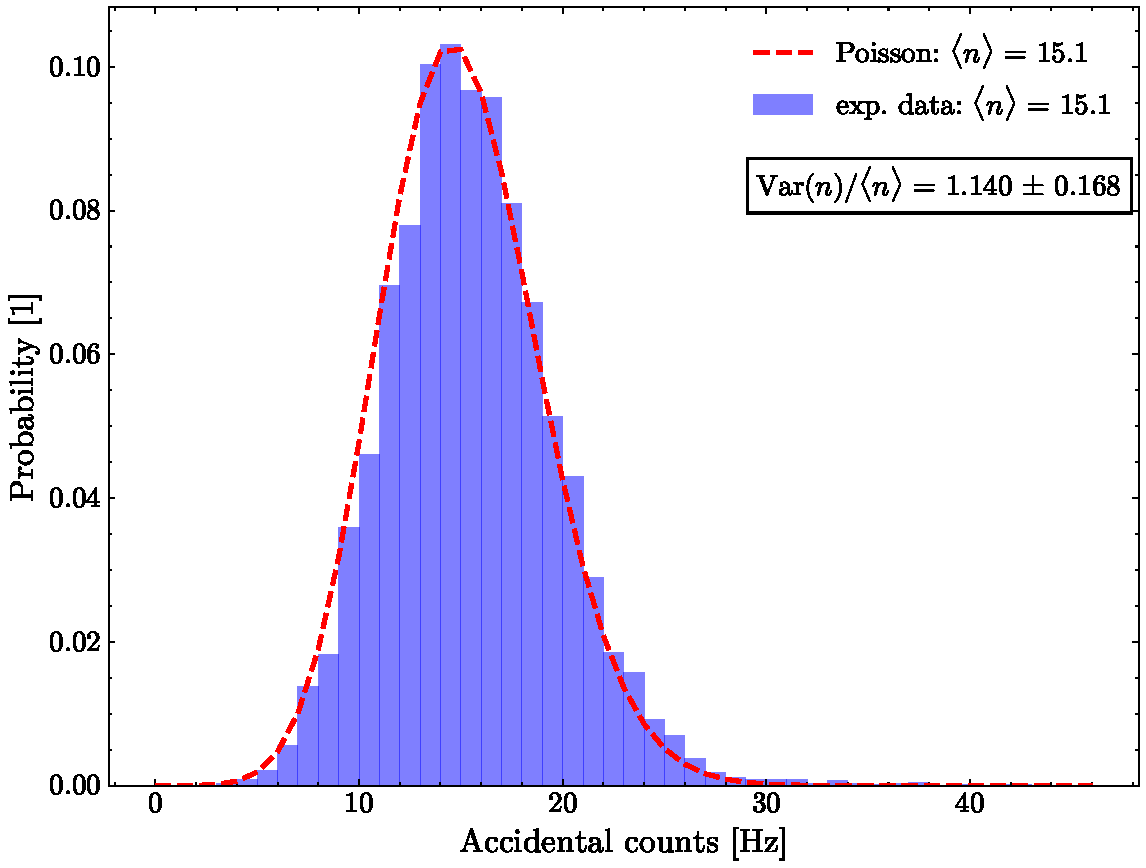
\includegraphics[width=.7\textwidth]{Images/AccCountsStatistics.pdf}
	\caption{Photon statistics of accidental counts}
	\label{fig:StatAcc}
\end{figure} \newline
Additionally, it has to be validated if the formula for calculating the accidentals in \autoref{eq:AccCounts} matches the experimental data. For this evaluation, histograms from the statistical analysis were used, as well as the single counts in each arm, i.e., the exposure time is one second and the integration time is sixty seconds. \newline
%The bin width was set to 1.4 ns and the coincidence window to 2.8 ns. \newline
According to \autoref{eq:AccCounts}, the accidental counts can be calculated at each time step using the single counts, coincidence counts and the coincidence window. This value is then compared with accidental counts measured experimentally. Again, in each time step, 105 values for the accidental counts were retrieved. In \autoref{fig:AccCompTheoExp}, the theoretical values are compared with the experimental ones, where for the experimental counts the average and standard deviation is shown. \newline
As can be seen, the theoretical values always fall within the standard deviation of the experimental ones. However, it is more important to consider whether the average value of the experimentally obtained counts can be well approximated by the formula, and thus, the theoretical values. This is decisive as the theoretical value obtained from \autoref{eq:AccCounts} is the estimator of the accidental counts in the transmittance model. 
\begin{figure}[tb!]
	\centering
	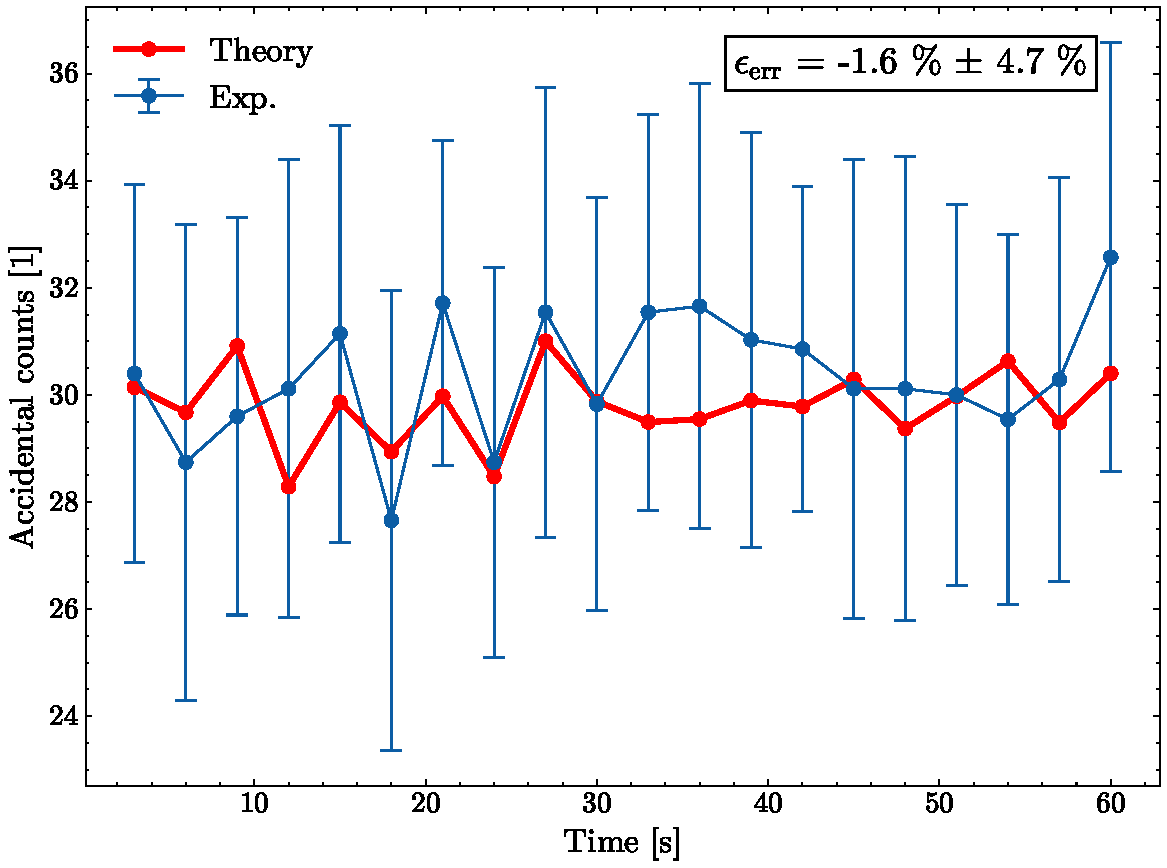
\includegraphics[width=.7\textwidth]{Images/AccCountsTheoExpRelError.pdf}
	\caption{Comparison between theoretically and experimentally obtained accidental counts}
	\label{fig:AccCompTheoExp}
\end{figure}\newline
To determine the deviation between the theoretical value and the average of the experimental accidental counts, the relative error was calculated at each time step as follows:
\begin{equation}
	\epsilon_{\text{err}} = \frac{R_{\text{acc}}^{\text{theo}}-R_{\text{acc}}^{\text{exp}}}{R_{\text{acc}}^{\text{exp}}}
\end{equation}
In the black box in \autoref{fig:AccCompTheoExp}, the mean value and standard deviation of the relative error for the sixty time steps is shown. As can be seen, the average relative error between the two values is 1.6 \%, so the formula can be used as a good approximation given the experimental uncertainties. \newline \newline
As a consequence, all parameters that are important for the transmittance model showed close agreement with the theoretical assumptions. As a next step, the approved model can be used to determine conditions in which the coincidence approach offers an advantage compared to the conventional one. 
\subsection{Heralding efficiencies}
Before applying the experimental results in the simulation, two more important parameters for the theoretical model need to be determined, which are the heralding efficiencies of each arm.\newline
They can be defined as the probability of detecting a photon in one arm given that a detection event has occurred in the other arm. For example, the heralding efficiency of the signal arm $\eta_{\text{sig}}$, conditioned on an idler detection, can be calculated using equations \ref{eq:SingleRef}, \ref{eq:pureCoinc} and \ref{eq:totCoinc}:
\begin{equation}
	\eta_{\text{sig}} = \frac{N_{\text{tot,cc}}-N_{\text{ac}}}{N_{\text{tot,idl}}-N_{\text{noise}}} = \frac{\eta_{\text{sig}}\eta_{\text{idl}}N_{\text{g}}}{\eta_{\text{idl}}N_{\text{g}}}
	\label{eq:EffSig}
\end{equation}
Analogously, the heralding efficiency of the idler arm $\eta_{\text{idl}}$, conditioned on the signal detection, is given by:
\begin{equation}
	\eta_{\text{idl}} = \frac{N_{\text{tot,cc}}-N_{\text{ac}}}{N_{\text{tot,sig}}-N_{\text{noise}}} = \frac{\eta_{\text{sig}}\eta_{\text{idl}}N_{\text{g}}}{\eta_{\text{sig}}N_{\text{g}}}
	\label{eq:EffIdl}
\end{equation}
It should be noted that the efficiency of the signal arm remains unchanged when a sample is placed in the idler arm. However, the efficiency of the idler arm itself decreases by a factor of $T$, the transmittance.\newline
Both heralding efficiencies are crucial to assess the quality of the experimental setup, as they provide direct information about optical loss in each arm. Efficiencies are also important when setting up the transmittance model, as they are crucial for analytically calculating coincidence and accidental counts.
\begin{figure}[tb!]
	\centering
	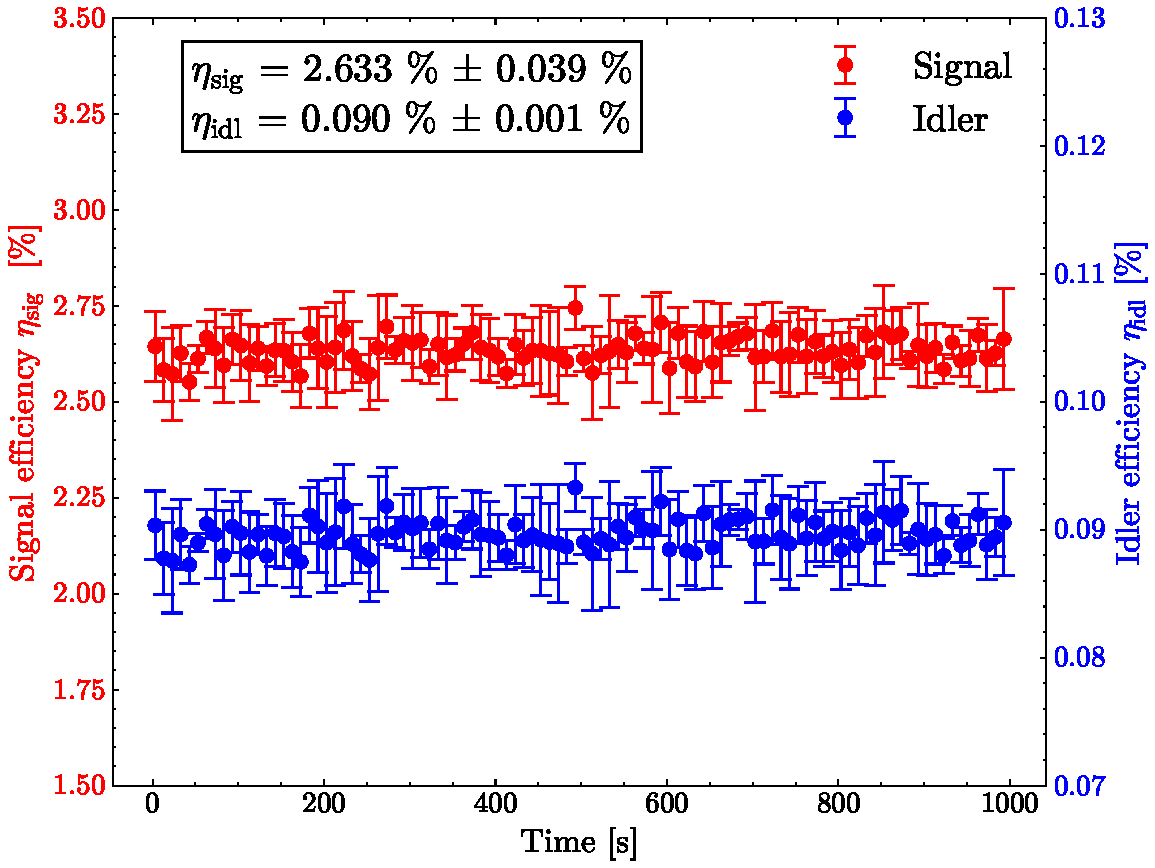
\includegraphics[width=.7\textwidth]{Images/HeraldingEff.pdf}
	\caption{Heralding efficiencies of the signal and idler arm}
	\label{fig:HeralEff}
\end{figure} \newline
Representative values for the efficiencies were measured experimentally in the setup as they will be used in the analytical formulas. The exposure time was set to one second and the integration time to one thousand seconds. At each time step, the single counts and histogram were retrieved, and the efficiencies were calculated using equations \ref{eq:EffSig} and \ref{eq:EffIdl}. The measurement was repeated six times to obtain a statistical distribution of the efficiencies. The results are shown in \autoref{fig:HeralEff}. \newline
As can be seen, the efficiency of the idler arm is much smaller than that of the signal arm, at 0.09\% and 2.63\% respectively. The reasons for this difference may be the alignment of both arms and the different efficiencies of the single-photon detectors. The average value of the efficiencies and their standard deviation is displayed in the black box. As can be seen, the fluctuations of both values are quite small. \newline
These two experimentally obtained efficiencies are used in the transmittance model to compare the conventional and coincidence approach in a simulation.



